\graphicspath{ {images/} }

\section{AXI4-Lite Fabric} \label{section_axi}

\subsection{Overview}
The configuration registers of Fire are configured via an AXI4-Lite
fabric, which is an industry standard interface for simple,
low-throughput register interfaces. Other low-throughput interfaces,
such as the side-path to OpenCAPI MMIO and Memory spaces, are also
part of this fabric. Xilinx FPGAs provide some optimizations for this
interface, and Xilinx IP utilizes AXI4-Lite heavily for configuration
and debug. This interface is illustrated in the overview picture in
Figure~\ref{fig:fire} and detailed in Figure ~\ref{fig:fire_axi}. The
AXI4-Lite fabric consists of three major components: an arbitrary
number of masters, an arbitrary number of slaves, and an AXI crossbar.

\begin{figure}[h]
  \begin{center}
    % Graphic for TeX using PGF
% Title: /home/rpking42/proj/chips/astra/doc/images/fire_axi.dia
% Creator: Dia v0.97.3
% CreationDate: Mon Aug 13 11:59:30 2018
% For: rpking42
% \usepackage{tikz}
% The following commands are not supported in PSTricks at present
% We define them conditionally, so when they are implemented,
% this pgf file will use them.
\ifx\du\undefined
  \newlength{\du}
\fi
\setlength{\du}{15\unitlength}
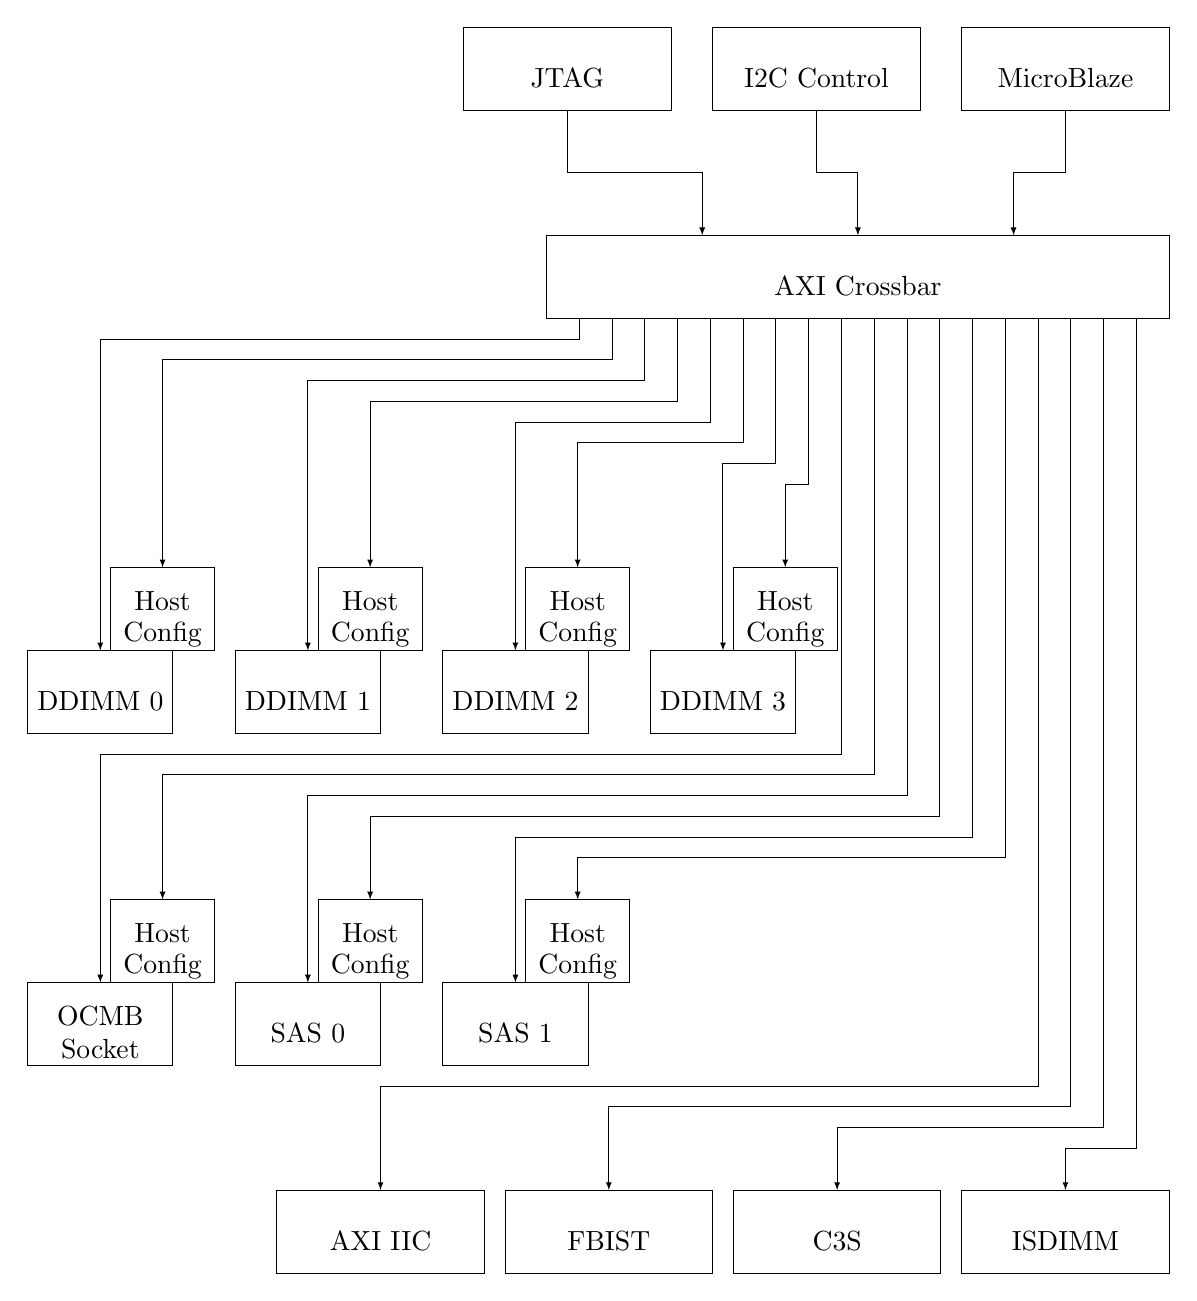
\begin{tikzpicture}
\pgftransformxscale{1.000000}
\pgftransformyscale{-1.000000}
\definecolor{dialinecolor}{rgb}{0.000000, 0.000000, 0.000000}
\pgfsetstrokecolor{dialinecolor}
\definecolor{dialinecolor}{rgb}{1.000000, 1.000000, 1.000000}
\pgfsetfillcolor{dialinecolor}
\pgfsetlinewidth{0.000000\du}
\pgfsetdash{}{0pt}
\pgfsetdash{}{0pt}
\pgfsetmiterjoin
\definecolor{dialinecolor}{rgb}{1.000000, 1.000000, 1.000000}
\pgfsetfillcolor{dialinecolor}
\fill (9.000000\du,25.000000\du)--(9.000000\du,27.000000\du)--(24.000000\du,27.000000\du)--(24.000000\du,25.000000\du)--cycle;
\definecolor{dialinecolor}{rgb}{0.000000, 0.000000, 0.000000}
\pgfsetstrokecolor{dialinecolor}
\draw (9.000000\du,25.000000\du)--(9.000000\du,27.000000\du)--(24.000000\du,27.000000\du)--(24.000000\du,25.000000\du)--cycle;
\pgfsetlinewidth{0.000000\du}
\pgfsetdash{}{0pt}
\pgfsetdash{}{0pt}
\pgfsetmiterjoin
\definecolor{dialinecolor}{rgb}{1.000000, 1.000000, 1.000000}
\pgfsetfillcolor{dialinecolor}
\fill (7.000000\du,20.000000\du)--(7.000000\du,22.000000\du)--(12.000000\du,22.000000\du)--(12.000000\du,20.000000\du)--cycle;
\definecolor{dialinecolor}{rgb}{0.000000, 0.000000, 0.000000}
\pgfsetstrokecolor{dialinecolor}
\draw (7.000000\du,20.000000\du)--(7.000000\du,22.000000\du)--(12.000000\du,22.000000\du)--(12.000000\du,20.000000\du)--cycle;
% setfont left to latex
\definecolor{dialinecolor}{rgb}{0.000000, 0.000000, 0.000000}
\pgfsetstrokecolor{dialinecolor}
\node at (9.500000\du,21.221250\du){JTAG};
\pgfsetlinewidth{0.000000\du}
\pgfsetdash{}{0pt}
\pgfsetdash{}{0pt}
\pgfsetmiterjoin
\pgfsetbuttcap
{
\definecolor{dialinecolor}{rgb}{0.000000, 0.000000, 0.000000}
\pgfsetfillcolor{dialinecolor}
% was here!!!
\pgfsetarrowsend{latex}
{\pgfsetcornersarced{\pgfpoint{0.000000\du}{0.000000\du}}\definecolor{dialinecolor}{rgb}{0.000000, 0.000000, 0.000000}
\pgfsetstrokecolor{dialinecolor}
\draw (9.500000\du,22.000000\du)--(9.500000\du,23.500000\du)--(12.750000\du,23.500000\du)--(12.750000\du,25.000000\du);
}}
\pgfsetlinewidth{0.000000\du}
\pgfsetdash{}{0pt}
\pgfsetdash{}{0pt}
\pgfsetmiterjoin
\definecolor{dialinecolor}{rgb}{1.000000, 1.000000, 1.000000}
\pgfsetfillcolor{dialinecolor}
\fill (13.000000\du,20.000000\du)--(13.000000\du,22.000000\du)--(18.000000\du,22.000000\du)--(18.000000\du,20.000000\du)--cycle;
\definecolor{dialinecolor}{rgb}{0.000000, 0.000000, 0.000000}
\pgfsetstrokecolor{dialinecolor}
\draw (13.000000\du,20.000000\du)--(13.000000\du,22.000000\du)--(18.000000\du,22.000000\du)--(18.000000\du,20.000000\du)--cycle;
% setfont left to latex
\definecolor{dialinecolor}{rgb}{0.000000, 0.000000, 0.000000}
\pgfsetstrokecolor{dialinecolor}
\node at (15.500000\du,21.221250\du){I2C Control};
\pgfsetlinewidth{0.000000\du}
\pgfsetdash{}{0pt}
\pgfsetdash{}{0pt}
\pgfsetmiterjoin
\definecolor{dialinecolor}{rgb}{1.000000, 1.000000, 1.000000}
\pgfsetfillcolor{dialinecolor}
\fill (19.000000\du,20.000000\du)--(19.000000\du,22.000000\du)--(24.000000\du,22.000000\du)--(24.000000\du,20.000000\du)--cycle;
\definecolor{dialinecolor}{rgb}{0.000000, 0.000000, 0.000000}
\pgfsetstrokecolor{dialinecolor}
\draw (19.000000\du,20.000000\du)--(19.000000\du,22.000000\du)--(24.000000\du,22.000000\du)--(24.000000\du,20.000000\du)--cycle;
% setfont left to latex
\definecolor{dialinecolor}{rgb}{0.000000, 0.000000, 0.000000}
\pgfsetstrokecolor{dialinecolor}
\node at (21.500000\du,21.221250\du){MicroBlaze};
\pgfsetlinewidth{0.000000\du}
\pgfsetdash{}{0pt}
\pgfsetdash{}{0pt}
\pgfsetmiterjoin
\pgfsetbuttcap
{
\definecolor{dialinecolor}{rgb}{0.000000, 0.000000, 0.000000}
\pgfsetfillcolor{dialinecolor}
% was here!!!
\pgfsetarrowsend{latex}
{\pgfsetcornersarced{\pgfpoint{0.000000\du}{0.000000\du}}\definecolor{dialinecolor}{rgb}{0.000000, 0.000000, 0.000000}
\pgfsetstrokecolor{dialinecolor}
\draw (15.500000\du,22.000000\du)--(15.500000\du,23.500000\du)--(16.500000\du,23.500000\du)--(16.500000\du,25.000000\du);
}}
\pgfsetlinewidth{0.000000\du}
\pgfsetdash{}{0pt}
\pgfsetdash{}{0pt}
\pgfsetbuttcap
{
\definecolor{dialinecolor}{rgb}{0.000000, 0.000000, 0.000000}
\pgfsetfillcolor{dialinecolor}
% was here!!!
\definecolor{dialinecolor}{rgb}{0.000000, 0.000000, 0.000000}
\pgfsetstrokecolor{dialinecolor}
\draw (9.000000\du,25.000000\du)--(24.000000\du,25.000000\du);
}
\pgfsetlinewidth{0.000000\du}
\pgfsetdash{}{0pt}
\pgfsetdash{}{0pt}
\pgfsetmiterjoin
\pgfsetbuttcap
{
\definecolor{dialinecolor}{rgb}{0.000000, 0.000000, 0.000000}
\pgfsetfillcolor{dialinecolor}
% was here!!!
\pgfsetarrowsend{latex}
{\pgfsetcornersarced{\pgfpoint{0.000000\du}{0.000000\du}}\definecolor{dialinecolor}{rgb}{0.000000, 0.000000, 0.000000}
\pgfsetstrokecolor{dialinecolor}
\draw (21.500000\du,22.000000\du)--(21.500000\du,23.500000\du)--(20.250000\du,23.500000\du)--(20.250000\du,25.000000\du);
}}
% setfont left to latex
\definecolor{dialinecolor}{rgb}{0.000000, 0.000000, 0.000000}
\pgfsetstrokecolor{dialinecolor}
\node at (16.500000\du,26.221250\du){AXI Crossbar};
\pgfsetlinewidth{0.000000\du}
\pgfsetdash{}{0pt}
\pgfsetdash{}{0pt}
\pgfsetmiterjoin
\definecolor{dialinecolor}{rgb}{1.000000, 1.000000, 1.000000}
\pgfsetfillcolor{dialinecolor}
\fill (13.500000\du,48.000000\du)--(13.500000\du,50.000000\du)--(18.500000\du,50.000000\du)--(18.500000\du,48.000000\du)--cycle;
\definecolor{dialinecolor}{rgb}{0.000000, 0.000000, 0.000000}
\pgfsetstrokecolor{dialinecolor}
\draw (13.500000\du,48.000000\du)--(13.500000\du,50.000000\du)--(18.500000\du,50.000000\du)--(18.500000\du,48.000000\du)--cycle;
% setfont left to latex
\definecolor{dialinecolor}{rgb}{0.000000, 0.000000, 0.000000}
\pgfsetstrokecolor{dialinecolor}
\node at (16.000000\du,49.221250\du){C3S};
\pgfsetlinewidth{0.000000\du}
\pgfsetdash{}{0pt}
\pgfsetdash{}{0pt}
\pgfsetmiterjoin
\definecolor{dialinecolor}{rgb}{1.000000, 1.000000, 1.000000}
\pgfsetfillcolor{dialinecolor}
\fill (19.000000\du,48.000000\du)--(19.000000\du,50.000000\du)--(24.000000\du,50.000000\du)--(24.000000\du,48.000000\du)--cycle;
\definecolor{dialinecolor}{rgb}{0.000000, 0.000000, 0.000000}
\pgfsetstrokecolor{dialinecolor}
\draw (19.000000\du,48.000000\du)--(19.000000\du,50.000000\du)--(24.000000\du,50.000000\du)--(24.000000\du,48.000000\du)--cycle;
% setfont left to latex
\definecolor{dialinecolor}{rgb}{0.000000, 0.000000, 0.000000}
\pgfsetstrokecolor{dialinecolor}
\node at (21.500000\du,49.221250\du){ISDIMM};
\pgfsetlinewidth{0.000000\du}
\pgfsetdash{}{0pt}
\pgfsetdash{}{0pt}
\pgfsetmiterjoin
\definecolor{dialinecolor}{rgb}{1.000000, 1.000000, 1.000000}
\pgfsetfillcolor{dialinecolor}
\fill (8.000000\du,48.000000\du)--(8.000000\du,50.000000\du)--(13.000000\du,50.000000\du)--(13.000000\du,48.000000\du)--cycle;
\definecolor{dialinecolor}{rgb}{0.000000, 0.000000, 0.000000}
\pgfsetstrokecolor{dialinecolor}
\draw (8.000000\du,48.000000\du)--(8.000000\du,50.000000\du)--(13.000000\du,50.000000\du)--(13.000000\du,48.000000\du)--cycle;
% setfont left to latex
\definecolor{dialinecolor}{rgb}{0.000000, 0.000000, 0.000000}
\pgfsetstrokecolor{dialinecolor}
\node at (10.500000\du,49.221250\du){FBIST};
\pgfsetlinewidth{0.000000\du}
\pgfsetdash{}{0pt}
\pgfsetdash{}{0pt}
\pgfsetmiterjoin
\definecolor{dialinecolor}{rgb}{1.000000, 1.000000, 1.000000}
\pgfsetfillcolor{dialinecolor}
\fill (2.500000\du,48.000000\du)--(2.500000\du,50.000000\du)--(7.500000\du,50.000000\du)--(7.500000\du,48.000000\du)--cycle;
\definecolor{dialinecolor}{rgb}{0.000000, 0.000000, 0.000000}
\pgfsetstrokecolor{dialinecolor}
\draw (2.500000\du,48.000000\du)--(2.500000\du,50.000000\du)--(7.500000\du,50.000000\du)--(7.500000\du,48.000000\du)--cycle;
% setfont left to latex
\definecolor{dialinecolor}{rgb}{0.000000, 0.000000, 0.000000}
\pgfsetstrokecolor{dialinecolor}
\node at (5.000000\du,49.221250\du){AXI IIC};
\pgfsetlinewidth{0.000000\du}
\pgfsetdash{}{0pt}
\pgfsetdash{}{0pt}
\pgfsetbuttcap
{
\definecolor{dialinecolor}{rgb}{0.000000, 0.000000, 0.000000}
\pgfsetfillcolor{dialinecolor}
% was here!!!
\definecolor{dialinecolor}{rgb}{0.000000, 0.000000, 0.000000}
\pgfsetstrokecolor{dialinecolor}
\draw (9.000000\du,27.000000\du)--(24.000000\du,27.000000\du);
}
\pgfsetlinewidth{0.000000\du}
\pgfsetdash{}{0pt}
\pgfsetdash{}{0pt}
\pgfsetmiterjoin
\pgfsetbuttcap
{
\definecolor{dialinecolor}{rgb}{0.000000, 0.000000, 0.000000}
\pgfsetfillcolor{dialinecolor}
% was here!!!
\pgfsetarrowsend{latex}
{\pgfsetcornersarced{\pgfpoint{0.000000\du}{0.000000\du}}\definecolor{dialinecolor}{rgb}{0.000000, 0.000000, 0.000000}
\pgfsetstrokecolor{dialinecolor}
\draw (23.210526\du,27.000000\du)--(23.210526\du,47.000000\du)--(21.500000\du,47.000000\du)--(21.500000\du,48.000000\du);
}}
\pgfsetlinewidth{0.000000\du}
\pgfsetdash{}{0pt}
\pgfsetdash{}{0pt}
\pgfsetmiterjoin
\pgfsetbuttcap
{
\definecolor{dialinecolor}{rgb}{0.000000, 0.000000, 0.000000}
\pgfsetfillcolor{dialinecolor}
% was here!!!
\pgfsetarrowsend{latex}
{\pgfsetcornersarced{\pgfpoint{0.000000\du}{0.000000\du}}\definecolor{dialinecolor}{rgb}{0.000000, 0.000000, 0.000000}
\pgfsetstrokecolor{dialinecolor}
\draw (22.421053\du,27.000000\du)--(22.421053\du,46.500000\du)--(16.000000\du,46.500000\du)--(16.000000\du,48.001465\du);
}}
\pgfsetlinewidth{0.000000\du}
\pgfsetdash{}{0pt}
\pgfsetdash{}{0pt}
\pgfsetmiterjoin
\pgfsetbuttcap
{
\definecolor{dialinecolor}{rgb}{0.000000, 0.000000, 0.000000}
\pgfsetfillcolor{dialinecolor}
% was here!!!
\pgfsetarrowsend{latex}
{\pgfsetcornersarced{\pgfpoint{0.000000\du}{0.000000\du}}\definecolor{dialinecolor}{rgb}{0.000000, 0.000000, 0.000000}
\pgfsetstrokecolor{dialinecolor}
\draw (21.631579\du,27.000000\du)--(21.631579\du,46.000000\du)--(10.500000\du,46.000000\du)--(10.500000\du,48.000244\du);
}}
\pgfsetlinewidth{0.000000\du}
\pgfsetdash{}{0pt}
\pgfsetdash{}{0pt}
\pgfsetmiterjoin
\pgfsetbuttcap
{
\definecolor{dialinecolor}{rgb}{0.000000, 0.000000, 0.000000}
\pgfsetfillcolor{dialinecolor}
% was here!!!
\pgfsetarrowsend{latex}
{\pgfsetcornersarced{\pgfpoint{0.000000\du}{0.000000\du}}\definecolor{dialinecolor}{rgb}{0.000000, 0.000000, 0.000000}
\pgfsetstrokecolor{dialinecolor}
\draw (20.842105\du,27.000000\du)--(20.842105\du,45.500000\du)--(5.000000\du,45.500000\du)--(5.000000\du,47.999817\du);
}}
\pgfsetlinewidth{0.000000\du}
\pgfsetdash{}{0pt}
\pgfsetdash{}{0pt}
\pgfsetmiterjoin
\definecolor{dialinecolor}{rgb}{1.000000, 1.000000, 1.000000}
\pgfsetfillcolor{dialinecolor}
\fill (-3.500000\du,35.000000\du)--(-3.500000\du,37.000000\du)--(0.000000\du,37.000000\du)--(0.000000\du,35.000000\du)--cycle;
\definecolor{dialinecolor}{rgb}{0.000000, 0.000000, 0.000000}
\pgfsetstrokecolor{dialinecolor}
\draw (-3.500000\du,35.000000\du)--(-3.500000\du,37.000000\du)--(0.000000\du,37.000000\du)--(0.000000\du,35.000000\du)--cycle;
% setfont left to latex
\definecolor{dialinecolor}{rgb}{0.000000, 0.000000, 0.000000}
\pgfsetstrokecolor{dialinecolor}
\node at (-1.750000\du,36.221250\du){DDIMM 0};
\pgfsetlinewidth{0.000000\du}
\pgfsetdash{}{0pt}
\pgfsetdash{}{0pt}
\pgfsetmiterjoin
\definecolor{dialinecolor}{rgb}{1.000000, 1.000000, 1.000000}
\pgfsetfillcolor{dialinecolor}
\fill (-1.500000\du,33.000000\du)--(-1.500000\du,35.000000\du)--(1.000000\du,35.000000\du)--(1.000000\du,33.000000\du)--cycle;
\definecolor{dialinecolor}{rgb}{0.000000, 0.000000, 0.000000}
\pgfsetstrokecolor{dialinecolor}
\draw (-1.500000\du,33.000000\du)--(-1.500000\du,35.000000\du)--(1.000000\du,35.000000\du)--(1.000000\du,33.000000\du)--cycle;
% setfont left to latex
\definecolor{dialinecolor}{rgb}{0.000000, 0.000000, 0.000000}
\pgfsetstrokecolor{dialinecolor}
\node at (-0.250000\du,33.821250\du){Host};
% setfont left to latex
\definecolor{dialinecolor}{rgb}{0.000000, 0.000000, 0.000000}
\pgfsetstrokecolor{dialinecolor}
\node at (-0.250000\du,34.621250\du){Config};
\pgfsetlinewidth{0.000000\du}
\pgfsetdash{}{0pt}
\pgfsetdash{}{0pt}
\pgfsetmiterjoin
\definecolor{dialinecolor}{rgb}{1.000000, 1.000000, 1.000000}
\pgfsetfillcolor{dialinecolor}
\fill (1.500000\du,35.000000\du)--(1.500000\du,37.000000\du)--(5.000000\du,37.000000\du)--(5.000000\du,35.000000\du)--cycle;
\definecolor{dialinecolor}{rgb}{0.000000, 0.000000, 0.000000}
\pgfsetstrokecolor{dialinecolor}
\draw (1.500000\du,35.000000\du)--(1.500000\du,37.000000\du)--(5.000000\du,37.000000\du)--(5.000000\du,35.000000\du)--cycle;
% setfont left to latex
\definecolor{dialinecolor}{rgb}{0.000000, 0.000000, 0.000000}
\pgfsetstrokecolor{dialinecolor}
\node at (3.250000\du,36.221250\du){DDIMM 1};
\pgfsetlinewidth{0.000000\du}
\pgfsetdash{}{0pt}
\pgfsetdash{}{0pt}
\pgfsetmiterjoin
\definecolor{dialinecolor}{rgb}{1.000000, 1.000000, 1.000000}
\pgfsetfillcolor{dialinecolor}
\fill (3.500000\du,33.000000\du)--(3.500000\du,35.000000\du)--(6.000000\du,35.000000\du)--(6.000000\du,33.000000\du)--cycle;
\definecolor{dialinecolor}{rgb}{0.000000, 0.000000, 0.000000}
\pgfsetstrokecolor{dialinecolor}
\draw (3.500000\du,33.000000\du)--(3.500000\du,35.000000\du)--(6.000000\du,35.000000\du)--(6.000000\du,33.000000\du)--cycle;
% setfont left to latex
\definecolor{dialinecolor}{rgb}{0.000000, 0.000000, 0.000000}
\pgfsetstrokecolor{dialinecolor}
\node at (4.750000\du,33.821250\du){Host};
% setfont left to latex
\definecolor{dialinecolor}{rgb}{0.000000, 0.000000, 0.000000}
\pgfsetstrokecolor{dialinecolor}
\node at (4.750000\du,34.621250\du){Config};
\pgfsetlinewidth{0.000000\du}
\pgfsetdash{}{0pt}
\pgfsetdash{}{0pt}
\pgfsetmiterjoin
\definecolor{dialinecolor}{rgb}{1.000000, 1.000000, 1.000000}
\pgfsetfillcolor{dialinecolor}
\fill (6.500000\du,35.000000\du)--(6.500000\du,37.000000\du)--(10.000000\du,37.000000\du)--(10.000000\du,35.000000\du)--cycle;
\definecolor{dialinecolor}{rgb}{0.000000, 0.000000, 0.000000}
\pgfsetstrokecolor{dialinecolor}
\draw (6.500000\du,35.000000\du)--(6.500000\du,37.000000\du)--(10.000000\du,37.000000\du)--(10.000000\du,35.000000\du)--cycle;
% setfont left to latex
\definecolor{dialinecolor}{rgb}{0.000000, 0.000000, 0.000000}
\pgfsetstrokecolor{dialinecolor}
\node at (8.250000\du,36.221250\du){DDIMM 2};
\pgfsetlinewidth{0.000000\du}
\pgfsetdash{}{0pt}
\pgfsetdash{}{0pt}
\pgfsetmiterjoin
\definecolor{dialinecolor}{rgb}{1.000000, 1.000000, 1.000000}
\pgfsetfillcolor{dialinecolor}
\fill (8.500000\du,33.000000\du)--(8.500000\du,35.000000\du)--(11.000000\du,35.000000\du)--(11.000000\du,33.000000\du)--cycle;
\definecolor{dialinecolor}{rgb}{0.000000, 0.000000, 0.000000}
\pgfsetstrokecolor{dialinecolor}
\draw (8.500000\du,33.000000\du)--(8.500000\du,35.000000\du)--(11.000000\du,35.000000\du)--(11.000000\du,33.000000\du)--cycle;
% setfont left to latex
\definecolor{dialinecolor}{rgb}{0.000000, 0.000000, 0.000000}
\pgfsetstrokecolor{dialinecolor}
\node at (9.750000\du,33.821250\du){Host};
% setfont left to latex
\definecolor{dialinecolor}{rgb}{0.000000, 0.000000, 0.000000}
\pgfsetstrokecolor{dialinecolor}
\node at (9.750000\du,34.621250\du){Config};
\pgfsetlinewidth{0.000000\du}
\pgfsetdash{}{0pt}
\pgfsetdash{}{0pt}
\pgfsetmiterjoin
\definecolor{dialinecolor}{rgb}{1.000000, 1.000000, 1.000000}
\pgfsetfillcolor{dialinecolor}
\fill (11.500000\du,35.000000\du)--(11.500000\du,37.000000\du)--(15.000000\du,37.000000\du)--(15.000000\du,35.000000\du)--cycle;
\definecolor{dialinecolor}{rgb}{0.000000, 0.000000, 0.000000}
\pgfsetstrokecolor{dialinecolor}
\draw (11.500000\du,35.000000\du)--(11.500000\du,37.000000\du)--(15.000000\du,37.000000\du)--(15.000000\du,35.000000\du)--cycle;
% setfont left to latex
\definecolor{dialinecolor}{rgb}{0.000000, 0.000000, 0.000000}
\pgfsetstrokecolor{dialinecolor}
\node at (13.250000\du,36.221250\du){DDIMM 3};
\pgfsetlinewidth{0.000000\du}
\pgfsetdash{}{0pt}
\pgfsetdash{}{0pt}
\pgfsetmiterjoin
\definecolor{dialinecolor}{rgb}{1.000000, 1.000000, 1.000000}
\pgfsetfillcolor{dialinecolor}
\fill (13.500000\du,33.000000\du)--(13.500000\du,35.000000\du)--(16.000000\du,35.000000\du)--(16.000000\du,33.000000\du)--cycle;
\definecolor{dialinecolor}{rgb}{0.000000, 0.000000, 0.000000}
\pgfsetstrokecolor{dialinecolor}
\draw (13.500000\du,33.000000\du)--(13.500000\du,35.000000\du)--(16.000000\du,35.000000\du)--(16.000000\du,33.000000\du)--cycle;
% setfont left to latex
\definecolor{dialinecolor}{rgb}{0.000000, 0.000000, 0.000000}
\pgfsetstrokecolor{dialinecolor}
\node at (14.750000\du,33.821250\du){Host};
% setfont left to latex
\definecolor{dialinecolor}{rgb}{0.000000, 0.000000, 0.000000}
\pgfsetstrokecolor{dialinecolor}
\node at (14.750000\du,34.621250\du){Config};
\pgfsetlinewidth{0.000000\du}
\pgfsetdash{}{0pt}
\pgfsetdash{}{0pt}
\pgfsetmiterjoin
\pgfsetbuttcap
{
\definecolor{dialinecolor}{rgb}{0.000000, 0.000000, 0.000000}
\pgfsetfillcolor{dialinecolor}
% was here!!!
\pgfsetarrowsend{latex}
{\pgfsetcornersarced{\pgfpoint{0.000000\du}{0.000000\du}}\definecolor{dialinecolor}{rgb}{0.000000, 0.000000, 0.000000}
\pgfsetstrokecolor{dialinecolor}
\draw (9.789474\du,27.000000\du)--(9.789474\du,27.500000\du)--(-1.750000\du,27.500000\du)--(-1.750000\du,35.000000\du);
}}
\pgfsetlinewidth{0.000000\du}
\pgfsetdash{}{0pt}
\pgfsetdash{}{0pt}
\pgfsetmiterjoin
\pgfsetbuttcap
{
\definecolor{dialinecolor}{rgb}{0.000000, 0.000000, 0.000000}
\pgfsetfillcolor{dialinecolor}
% was here!!!
\pgfsetarrowsend{latex}
{\pgfsetcornersarced{\pgfpoint{0.000000\du}{0.000000\du}}\definecolor{dialinecolor}{rgb}{0.000000, 0.000000, 0.000000}
\pgfsetstrokecolor{dialinecolor}
\draw (10.578947\du,27.000000\du)--(10.578947\du,28.000000\du)--(-0.250000\du,28.000000\du)--(-0.250000\du,33.000000\du);
}}
\pgfsetlinewidth{0.000000\du}
\pgfsetdash{}{0pt}
\pgfsetdash{}{0pt}
\pgfsetmiterjoin
\pgfsetbuttcap
{
\definecolor{dialinecolor}{rgb}{0.000000, 0.000000, 0.000000}
\pgfsetfillcolor{dialinecolor}
% was here!!!
\pgfsetarrowsend{latex}
{\pgfsetcornersarced{\pgfpoint{0.000000\du}{0.000000\du}}\definecolor{dialinecolor}{rgb}{0.000000, 0.000000, 0.000000}
\pgfsetstrokecolor{dialinecolor}
\draw (11.368421\du,27.000000\du)--(11.368421\du,28.500000\du)--(3.250000\du,28.500000\du)--(3.250000\du,35.000000\du);
}}
\pgfsetlinewidth{0.000000\du}
\pgfsetdash{}{0pt}
\pgfsetdash{}{0pt}
\pgfsetmiterjoin
\pgfsetbuttcap
{
\definecolor{dialinecolor}{rgb}{0.000000, 0.000000, 0.000000}
\pgfsetfillcolor{dialinecolor}
% was here!!!
\pgfsetarrowsend{latex}
{\pgfsetcornersarced{\pgfpoint{0.000000\du}{0.000000\du}}\definecolor{dialinecolor}{rgb}{0.000000, 0.000000, 0.000000}
\pgfsetstrokecolor{dialinecolor}
\draw (12.157895\du,27.000000\du)--(12.157895\du,29.000000\du)--(4.750000\du,29.000000\du)--(4.750000\du,33.000000\du);
}}
\pgfsetlinewidth{0.000000\du}
\pgfsetdash{}{0pt}
\pgfsetdash{}{0pt}
\pgfsetmiterjoin
\pgfsetbuttcap
{
\definecolor{dialinecolor}{rgb}{0.000000, 0.000000, 0.000000}
\pgfsetfillcolor{dialinecolor}
% was here!!!
\pgfsetarrowsend{latex}
{\pgfsetcornersarced{\pgfpoint{0.000000\du}{0.000000\du}}\definecolor{dialinecolor}{rgb}{0.000000, 0.000000, 0.000000}
\pgfsetstrokecolor{dialinecolor}
\draw (12.947368\du,27.000000\du)--(12.947368\du,29.500000\du)--(8.250000\du,29.500000\du)--(8.250000\du,35.000000\du);
}}
\pgfsetlinewidth{0.000000\du}
\pgfsetdash{}{0pt}
\pgfsetdash{}{0pt}
\pgfsetmiterjoin
\pgfsetbuttcap
{
\definecolor{dialinecolor}{rgb}{0.000000, 0.000000, 0.000000}
\pgfsetfillcolor{dialinecolor}
% was here!!!
\pgfsetarrowsend{latex}
{\pgfsetcornersarced{\pgfpoint{0.000000\du}{0.000000\du}}\definecolor{dialinecolor}{rgb}{0.000000, 0.000000, 0.000000}
\pgfsetstrokecolor{dialinecolor}
\draw (13.736842\du,27.000000\du)--(13.736842\du,30.000000\du)--(9.750000\du,30.000000\du)--(9.750000\du,33.000000\du);
}}
\pgfsetlinewidth{0.000000\du}
\pgfsetdash{}{0pt}
\pgfsetdash{}{0pt}
\pgfsetmiterjoin
\pgfsetbuttcap
{
\definecolor{dialinecolor}{rgb}{0.000000, 0.000000, 0.000000}
\pgfsetfillcolor{dialinecolor}
% was here!!!
\pgfsetarrowsend{latex}
{\pgfsetcornersarced{\pgfpoint{0.000000\du}{0.000000\du}}\definecolor{dialinecolor}{rgb}{0.000000, 0.000000, 0.000000}
\pgfsetstrokecolor{dialinecolor}
\draw (14.526316\du,27.000000\du)--(14.526316\du,30.500000\du)--(13.250000\du,30.500000\du)--(13.250000\du,35.000000\du);
}}
\pgfsetlinewidth{0.000000\du}
\pgfsetdash{}{0pt}
\pgfsetdash{}{0pt}
\pgfsetmiterjoin
\pgfsetbuttcap
{
\definecolor{dialinecolor}{rgb}{0.000000, 0.000000, 0.000000}
\pgfsetfillcolor{dialinecolor}
% was here!!!
\pgfsetarrowsend{latex}
{\pgfsetcornersarced{\pgfpoint{0.000000\du}{0.000000\du}}\definecolor{dialinecolor}{rgb}{0.000000, 0.000000, 0.000000}
\pgfsetstrokecolor{dialinecolor}
\draw (15.315789\du,27.000000\du)--(15.315789\du,31.000000\du)--(14.750000\du,31.000000\du)--(14.750000\du,33.000000\du);
}}
\pgfsetlinewidth{0.000000\du}
\pgfsetdash{}{0pt}
\pgfsetdash{}{0pt}
\pgfsetmiterjoin
\definecolor{dialinecolor}{rgb}{1.000000, 1.000000, 1.000000}
\pgfsetfillcolor{dialinecolor}
\fill (-3.500000\du,43.000000\du)--(-3.500000\du,45.000000\du)--(0.000000\du,45.000000\du)--(0.000000\du,43.000000\du)--cycle;
\definecolor{dialinecolor}{rgb}{0.000000, 0.000000, 0.000000}
\pgfsetstrokecolor{dialinecolor}
\draw (-3.500000\du,43.000000\du)--(-3.500000\du,45.000000\du)--(0.000000\du,45.000000\du)--(0.000000\du,43.000000\du)--cycle;
% setfont left to latex
\definecolor{dialinecolor}{rgb}{0.000000, 0.000000, 0.000000}
\pgfsetstrokecolor{dialinecolor}
\node at (-1.750000\du,43.811906\du){OCMB};
% setfont left to latex
\definecolor{dialinecolor}{rgb}{0.000000, 0.000000, 0.000000}
\pgfsetstrokecolor{dialinecolor}
\node at (-1.750000\du,44.611906\du){Socket};
\pgfsetlinewidth{0.000000\du}
\pgfsetdash{}{0pt}
\pgfsetdash{}{0pt}
\pgfsetmiterjoin
\definecolor{dialinecolor}{rgb}{1.000000, 1.000000, 1.000000}
\pgfsetfillcolor{dialinecolor}
\fill (-1.500000\du,41.000000\du)--(-1.500000\du,43.000000\du)--(1.000000\du,43.000000\du)--(1.000000\du,41.000000\du)--cycle;
\definecolor{dialinecolor}{rgb}{0.000000, 0.000000, 0.000000}
\pgfsetstrokecolor{dialinecolor}
\draw (-1.500000\du,41.000000\du)--(-1.500000\du,43.000000\du)--(1.000000\du,43.000000\du)--(1.000000\du,41.000000\du)--cycle;
% setfont left to latex
\definecolor{dialinecolor}{rgb}{0.000000, 0.000000, 0.000000}
\pgfsetstrokecolor{dialinecolor}
\node at (-0.250000\du,41.821250\du){Host};
% setfont left to latex
\definecolor{dialinecolor}{rgb}{0.000000, 0.000000, 0.000000}
\pgfsetstrokecolor{dialinecolor}
\node at (-0.250000\du,42.621250\du){Config};
\pgfsetlinewidth{0.000000\du}
\pgfsetdash{}{0pt}
\pgfsetdash{}{0pt}
\pgfsetmiterjoin
\definecolor{dialinecolor}{rgb}{1.000000, 1.000000, 1.000000}
\pgfsetfillcolor{dialinecolor}
\fill (1.500000\du,43.000000\du)--(1.500000\du,45.000000\du)--(5.000000\du,45.000000\du)--(5.000000\du,43.000000\du)--cycle;
\definecolor{dialinecolor}{rgb}{0.000000, 0.000000, 0.000000}
\pgfsetstrokecolor{dialinecolor}
\draw (1.500000\du,43.000000\du)--(1.500000\du,45.000000\du)--(5.000000\du,45.000000\du)--(5.000000\du,43.000000\du)--cycle;
% setfont left to latex
\definecolor{dialinecolor}{rgb}{0.000000, 0.000000, 0.000000}
\pgfsetstrokecolor{dialinecolor}
\node at (3.250000\du,44.221250\du){SAS 0};
\pgfsetlinewidth{0.000000\du}
\pgfsetdash{}{0pt}
\pgfsetdash{}{0pt}
\pgfsetmiterjoin
\definecolor{dialinecolor}{rgb}{1.000000, 1.000000, 1.000000}
\pgfsetfillcolor{dialinecolor}
\fill (3.500000\du,41.000000\du)--(3.500000\du,43.000000\du)--(6.000000\du,43.000000\du)--(6.000000\du,41.000000\du)--cycle;
\definecolor{dialinecolor}{rgb}{0.000000, 0.000000, 0.000000}
\pgfsetstrokecolor{dialinecolor}
\draw (3.500000\du,41.000000\du)--(3.500000\du,43.000000\du)--(6.000000\du,43.000000\du)--(6.000000\du,41.000000\du)--cycle;
% setfont left to latex
\definecolor{dialinecolor}{rgb}{0.000000, 0.000000, 0.000000}
\pgfsetstrokecolor{dialinecolor}
\node at (4.750000\du,41.821250\du){Host};
% setfont left to latex
\definecolor{dialinecolor}{rgb}{0.000000, 0.000000, 0.000000}
\pgfsetstrokecolor{dialinecolor}
\node at (4.750000\du,42.621250\du){Config};
\pgfsetlinewidth{0.000000\du}
\pgfsetdash{}{0pt}
\pgfsetdash{}{0pt}
\pgfsetmiterjoin
\definecolor{dialinecolor}{rgb}{1.000000, 1.000000, 1.000000}
\pgfsetfillcolor{dialinecolor}
\fill (6.500000\du,43.000000\du)--(6.500000\du,45.000000\du)--(10.000000\du,45.000000\du)--(10.000000\du,43.000000\du)--cycle;
\definecolor{dialinecolor}{rgb}{0.000000, 0.000000, 0.000000}
\pgfsetstrokecolor{dialinecolor}
\draw (6.500000\du,43.000000\du)--(6.500000\du,45.000000\du)--(10.000000\du,45.000000\du)--(10.000000\du,43.000000\du)--cycle;
% setfont left to latex
\definecolor{dialinecolor}{rgb}{0.000000, 0.000000, 0.000000}
\pgfsetstrokecolor{dialinecolor}
\node at (8.250000\du,44.221250\du){SAS 1};
\pgfsetlinewidth{0.000000\du}
\pgfsetdash{}{0pt}
\pgfsetdash{}{0pt}
\pgfsetmiterjoin
\definecolor{dialinecolor}{rgb}{1.000000, 1.000000, 1.000000}
\pgfsetfillcolor{dialinecolor}
\fill (8.500000\du,41.000000\du)--(8.500000\du,43.000000\du)--(11.000000\du,43.000000\du)--(11.000000\du,41.000000\du)--cycle;
\definecolor{dialinecolor}{rgb}{0.000000, 0.000000, 0.000000}
\pgfsetstrokecolor{dialinecolor}
\draw (8.500000\du,41.000000\du)--(8.500000\du,43.000000\du)--(11.000000\du,43.000000\du)--(11.000000\du,41.000000\du)--cycle;
% setfont left to latex
\definecolor{dialinecolor}{rgb}{0.000000, 0.000000, 0.000000}
\pgfsetstrokecolor{dialinecolor}
\node at (9.750000\du,41.821250\du){Host};
% setfont left to latex
\definecolor{dialinecolor}{rgb}{0.000000, 0.000000, 0.000000}
\pgfsetstrokecolor{dialinecolor}
\node at (9.750000\du,42.621250\du){Config};
\pgfsetlinewidth{0.000000\du}
\pgfsetdash{}{0pt}
\pgfsetdash{}{0pt}
\pgfsetmiterjoin
\pgfsetbuttcap
{
\definecolor{dialinecolor}{rgb}{0.000000, 0.000000, 0.000000}
\pgfsetfillcolor{dialinecolor}
% was here!!!
\pgfsetarrowsend{latex}
{\pgfsetcornersarced{\pgfpoint{0.000000\du}{0.000000\du}}\definecolor{dialinecolor}{rgb}{0.000000, 0.000000, 0.000000}
\pgfsetstrokecolor{dialinecolor}
\draw (16.105263\du,27.000000\du)--(16.105263\du,37.500000\du)--(-1.750000\du,37.500000\du)--(-1.750000\du,43.000000\du);
}}
\pgfsetlinewidth{0.000000\du}
\pgfsetdash{}{0pt}
\pgfsetdash{}{0pt}
\pgfsetmiterjoin
\pgfsetbuttcap
{
\definecolor{dialinecolor}{rgb}{0.000000, 0.000000, 0.000000}
\pgfsetfillcolor{dialinecolor}
% was here!!!
\pgfsetarrowsend{latex}
{\pgfsetcornersarced{\pgfpoint{0.000000\du}{0.000000\du}}\definecolor{dialinecolor}{rgb}{0.000000, 0.000000, 0.000000}
\pgfsetstrokecolor{dialinecolor}
\draw (16.894737\du,27.000000\du)--(16.894737\du,38.000000\du)--(-0.250000\du,38.000000\du)--(-0.250000\du,41.000000\du);
}}
\pgfsetlinewidth{0.000000\du}
\pgfsetdash{}{0pt}
\pgfsetdash{}{0pt}
\pgfsetmiterjoin
\pgfsetbuttcap
{
\definecolor{dialinecolor}{rgb}{0.000000, 0.000000, 0.000000}
\pgfsetfillcolor{dialinecolor}
% was here!!!
\pgfsetarrowsend{latex}
{\pgfsetcornersarced{\pgfpoint{0.000000\du}{0.000000\du}}\definecolor{dialinecolor}{rgb}{0.000000, 0.000000, 0.000000}
\pgfsetstrokecolor{dialinecolor}
\draw (17.684211\du,27.000000\du)--(17.684211\du,38.500000\du)--(3.250000\du,38.500000\du)--(3.250000\du,43.000000\du);
}}
\pgfsetlinewidth{0.000000\du}
\pgfsetdash{}{0pt}
\pgfsetdash{}{0pt}
\pgfsetmiterjoin
\pgfsetbuttcap
{
\definecolor{dialinecolor}{rgb}{0.000000, 0.000000, 0.000000}
\pgfsetfillcolor{dialinecolor}
% was here!!!
\pgfsetarrowsend{latex}
{\pgfsetcornersarced{\pgfpoint{0.000000\du}{0.000000\du}}\definecolor{dialinecolor}{rgb}{0.000000, 0.000000, 0.000000}
\pgfsetstrokecolor{dialinecolor}
\draw (18.473684\du,27.000000\du)--(18.473684\du,39.000000\du)--(4.750000\du,39.000000\du)--(4.750000\du,41.000000\du);
}}
\pgfsetlinewidth{0.000000\du}
\pgfsetdash{}{0pt}
\pgfsetdash{}{0pt}
\pgfsetmiterjoin
\pgfsetbuttcap
{
\definecolor{dialinecolor}{rgb}{0.000000, 0.000000, 0.000000}
\pgfsetfillcolor{dialinecolor}
% was here!!!
\pgfsetarrowsend{latex}
{\pgfsetcornersarced{\pgfpoint{0.000000\du}{0.000000\du}}\definecolor{dialinecolor}{rgb}{0.000000, 0.000000, 0.000000}
\pgfsetstrokecolor{dialinecolor}
\draw (19.263158\du,27.000000\du)--(19.263158\du,39.500000\du)--(8.250000\du,39.500000\du)--(8.250000\du,42.999695\du);
}}
\pgfsetlinewidth{0.000000\du}
\pgfsetdash{}{0pt}
\pgfsetdash{}{0pt}
\pgfsetmiterjoin
\pgfsetbuttcap
{
\definecolor{dialinecolor}{rgb}{0.000000, 0.000000, 0.000000}
\pgfsetfillcolor{dialinecolor}
% was here!!!
\pgfsetarrowsend{latex}
{\pgfsetcornersarced{\pgfpoint{0.000000\du}{0.000000\du}}\definecolor{dialinecolor}{rgb}{0.000000, 0.000000, 0.000000}
\pgfsetstrokecolor{dialinecolor}
\draw (20.052632\du,27.000000\du)--(20.052632\du,40.000000\du)--(9.750000\du,40.000000\du)--(9.750000\du,41.000000\du);
}}
\end{tikzpicture}

  \end{center}
  \caption[AXI Fabric]{\label{fig:fire_axi}AXI Fabric
  }
\end{figure}

Fire has the following components that act as AXI4-Lite masters (2 total):
\begin{itemize}
  \item JTAG/AXI Bridge
  \item I2C Control
\end{itemize}
Each of these masters has full access to all slaves on the interface,
with each slave having the same address offset in each case. The
JTAG/AXI bridge is accessed only from Vivado, while the I2C Control
handles I2C commands passed into the chip from another I2C Master.

The following components act as AXI4-Lite slaves (32 total):
\begin{itemize}
  \item DDIMM 0-3 (MMIO space, Config Space, and Real Memory)
  \item Explorer Socket (MMIO space, Config Space, and Real Memory)
  \item SlimSAS 0-1 (MMIO space, Config Space, and Real Memory)
  \item ISDIMM
  \item C3S
  \item FBIST
  \item AXI IIC
  \item OpenCAPI TL Host Configuration (Links for DDIMM 0-3, Socket, SlimSAS 0-1)
\end{itemize}
C3S and FBIST have configuration registers programmed over
AXI4-Lite. In both of these components, a test is programmed and then
started via AXI, and then commands are driven directly to the OpenCAPI
link. For the ISDIMM, controlled by a Xilinx DDR4 MIG, the DDR4 memory
can be written with arbitrary information and then read out
later. Finally, each OpenCAPI link has 4 register spaces associated
with it: MMIO space, Config Space, Real Memory Space, and Host
Configuration. For the first three, The OpenCAPI TL accepts an
AXI4-Lite interface. This is separate from the AXI4 interface driven
by FBIST. The AXI4-Lite interface serves as a means to read and write
registers or memory in OCMB, at a very low throughput, but with a
simple interface. The Host Configuration has a small number of
registers that control how the OpenCAPI link functions on the host
side.

The crossbar is Xilinx IP that serves as an arbiter among the multiple
masters. It also looks at the configured address space to direct an
AXI transaction to the appropriate slave.

Between each master/slave and the crossbar is also a number of stages
of pipelining and/or an asynchronous boundary. AXI allows all masters
and slaves to run at different speeds. Although this isn't
functionally required, it can help ease timing requirements as this
fabric spreads throughout the chip. Even if there is not a clock
domain crossing, pipeline stages may be added to easy timing as
well. Because AXI is not a high performance interface, this increases
latency an acceptable amount to ease implementation. These blocks are
inserted in both directions. If there is an asynchronous crossing or
pipeline stages, it is indicated in Figure ~\ref{fig:fire_axi}.

\subsection{Address Map}
The address map indicates where in the global address space a memory
address is located. The global space includes all registers and memory
on Apollo, which includes the FPGA as well as all attached OCMBs. The
AXI Fabric identifies which macro an address is in, and then directs
the AXI transaction to that slave. The slave then uses the mask for
its memory size to extract the local address. For example, C3S has a
24-bit local address, while the MMIO space on a DDIMM has a 32-bit
local address. Inside Fire, bits of the address are little endian,
address(63 downto 0).

When assembling the address space, several bits were chosen to have
significant meaning. These can be found in the address table below,
but some are explained here. Bit 56, the Chip (C) bit indicates
whether the memory space is in Fire (1) or in OCMB (0). For spaces in
Fire, bits 51:48 indicate the macro. For spaces in OCMB, bits 51:49
indicate the method being used (config, MMIO, or real memory). In both
chips, if an address space is duplicated among multiple OpenCAPI ports
(e.g. MMIO or Host Config), bits 47:42 indicate which OCMB.

Address sizes were chosen incredibly generously, and it is not
expected that any address space will ever become close to being
exhausted.

The first 4 bits of each address, as sent over i2c to Fire, is an
encoded length of the data associated with the read or write, and is
not part of the actual address. The 4 MSB bits of the address should
be set to 0 before doing any address mapping. The encoded lengths are as follows:


\begin{table}[h]
  \begin{center}
    \begin{tabular}{ c | l }
      Address Encoding & Operation Length \\
      \hline
      \texttt{0b0000}  & 1 byte           \\
      \texttt{0b0001}  & 2 bytes          \\
      \texttt{0b0010}  & 4 bytes          \\
      \texttt{0b0011}  & 8 bytes          \\
      \texttt{0b0100}  & 16 bytes         \\
      \texttt{0b0101}  & 32 bytes         \\
      \texttt{0b0110}  & 64 bytes         \\
      \texttt{0b0111}  & 128 bytes        \\
      \texttt{0b1000}  & 256 bytes        \\
      Others           & Reserved         \\
    \end{tabular}
  \end{center}
  \textbf{Note}: Only 4 byte and 8 byte operations are used, other decode points are for future expansion
  \caption[Length Encoding of 4 MSB of I2C address]{\label{table:i2c_address_length_encoding}Length Encoding of 4 MSB of I2C address
  }
\end{table}

\begin{landscape}
  \begin{table}[h]
    \begin{center}
      \begin{tabular}{ l | c | c | r | c | l }
        Macro                 & Address Start                     & Address End                       & Size   & Protocol  & Interface \\
        \hline
        DDIMM 0 Memory        & \texttt{0x0000\_0000\_0000\_0000} & \texttt{0x0000\_03FF\_FFFF\_FFFF} & 4 TB   & AXI3      & M1        \\
        DDIMM 1 Memory        & \texttt{0x0000\_0400\_0000\_0000} & \texttt{0x0000\_07FF\_FFFF\_FFFF} & 4 TB   & AXI3      & M4        \\
        DDIMM 2 Memory        & \texttt{0x0000\_0800\_0000\_0000} & \texttt{0x0000\_0BFF\_FFFF\_FFFF} & 4 TB   & AXI3      & M7        \\
        DDIMM 3 Memory        & \texttt{0x0000\_0C00\_0000\_0000} & \texttt{0x0000\_0FFF\_FFFF\_FFFF} & 4 TB   & AXI3      & M10       \\
%       Socket Memory         & \texttt{0x0000\_1000\_0000\_0000} & \texttt{0x0000\_13FF\_FFFF\_FFFF} & 4 TB   & AXI3      & M13       \\
%       SlimSAS 0 Memory      & \texttt{0x0000\_1400\_0000\_0000} & \texttt{0x0000\_17FF\_FFFF\_FFFF} & 4 TB   & AXI3      & M16       \\
%       SlimSAS 1 Memory      & \texttt{0x0000\_1800\_0000\_0000} & \texttt{0x0000\_1BFF\_FFFF\_FFFF} & 4 TB   & AXI3      & M19       \\
        DDIMM 0 CFG           & \texttt{0x0001\_0000\_0000\_0000} & \texttt{0x0001\_0000\_7FFF\_FFFF} & 2 GB   & AXI3      & M3        \\
        DDIMM 1 CFG           & \texttt{0x0001\_0400\_0000\_0000} & \texttt{0x0001\_0400\_7FFF\_FFFF} & 2 GB   & AXI3      & M6        \\
        DDIMM 2 CFG           & \texttt{0x0001\_0800\_0000\_0000} & \texttt{0x0001\_0800\_7FFF\_FFFF} & 2 GB   & AXI3      & M9        \\
        DDIMM 3 CFG           & \texttt{0x0001\_0C00\_0000\_0000} & \texttt{0x0001\_0C00\_7FFF\_FFFF} & 2 GB   & AXI3      & M12       \\
%       Socket CFG            & \texttt{0x0001\_1000\_0000\_0000} & \texttt{0x0001\_1000\_7FFF\_FFFF} & 2 GB   & AXI3      & M15       \\
%       SlimSAS 0 CFG         & \texttt{0x0001\_1400\_0000\_0000} & \texttt{0x0001\_1400\_7FFF\_FFFF} & 2 GB   & AXI3      & M18       \\
%       SlimSAS 1 CFG         & \texttt{0x0001\_1800\_0000\_0000} & \texttt{0x0001\_1800\_7FFF\_FFFF} & 2 GB   & AXI3      & M21       \\
        DDIMM 0 MMIO          & \texttt{0x0001\_0001\_0000\_0000} & \texttt{0x0001\_0001\_7FFF\_FFFF} & 2 GB   & AXI3      & M2        \\
        DDIMM 1 MMIO          & \texttt{0x0001\_0401\_0000\_0000} & \texttt{0x0001\_0401\_7FFF\_FFFF} & 2 GB   & AXI3      & M5        \\
        DDIMM 2 MMIO          & \texttt{0x0001\_0801\_0000\_0000} & \texttt{0x0001\_0801\_7FFF\_FFFF} & 2 GB   & AXI3      & M8        \\
        DDIMM 3 MMIO          & \texttt{0x0001\_0C01\_0000\_0000} & \texttt{0x0001\_0C01\_7FFF\_FFFF} & 2 GB   & AXI3      & M11       \\
%       Socket MMIO           & \texttt{0x0001\_1001\_0000\_0000} & \texttt{0x0001\_1001\_7FFF\_FFFF} & 2 GB   & AXI3      & M14       \\
%       SlimSAS 0 MMIO        & \texttt{0x0001\_1401\_0000\_0000} & \texttt{0x0001\_1401\_7FFF\_FFFF} & 2 GB   & AXI3      & M17       \\
%       SlimSAS 1 MMIO        & \texttt{0x0001\_1801\_0000\_0000} & \texttt{0x0001\_1801\_7FFF\_FFFF} & 2 GB   & AXI3      & M20       \\
        FML                   & \texttt{0x0100\_0000\_0000\_0000} & \texttt{0x0100\_0000\_00FF\_FFFF} & 16 MB  & AXI4-Lite & M0        \\
        DDIMM 0 C3S           & \texttt{0x0101\_0000\_0000\_0000} & \texttt{0x0101\_0000\_00FF\_FFFF} & 16 MB  & AXI4-Lite & M1        \\
        DDIMM 1 C3S           & \texttt{0x0101\_0400\_0000\_0000} & \texttt{0x0101\_0400\_00FF\_FFFF} & 16 MB  & AXI4-Lite & M9        \\
        DDIMM 2 C3S           & \texttt{0x0101\_0800\_0000\_0000} & \texttt{0x0101\_0800\_00FF\_FFFF} & 16 MB  & AXI4-Lite & M11       \\
        DDIMM 3 C3S           & \texttt{0x0101\_0C00\_0000\_0000} & \texttt{0x0101\_0C00\_00FF\_FFFF} & 16 MB  & AXI4-Lite & M13       \\
%       Socket C3S            & \texttt{0x0101\_1000\_0000\_0000} & \texttt{0x0101\_1000\_00FF\_FFFF} & 16 MB  & AXI4-Lite & M15       \\
%       SlimSAS 0 C3S         & \texttt{0x0101\_1400\_0000\_0000} & \texttt{0x0101\_1400\_00FF\_FFFF} & 16 MB  & AXI4-Lite & M17       \\
%       SlimSAS 1 C3S         & \texttt{0x0101\_1800\_0000\_0000} & \texttt{0x0101\_1800\_00FF\_FFFF} & 16 MB  & AXI4-Lite & M19       \\
        DDIMM 0 FBIST         & \texttt{0x0102\_0000\_0000\_0000} & \texttt{0x0102\_0000\_00FF\_FFFF} & 16 MB  & AXI4-Lite & M2        \\
        DDIMM 1 FBIST         & \texttt{0x0102\_0400\_0000\_0000} & \texttt{0x0102\_0400\_00FF\_FFFF} & 16 MB  & AXI4-Lite & M10       \\
        DDIMM 2 FBIST         & \texttt{0x0102\_0800\_0000\_0000} & \texttt{0x0102\_0800\_00FF\_FFFF} & 16 MB  & AXI4-Lite & M12       \\
        DDIMM 3 FBIST         & \texttt{0x0102\_0C00\_0000\_0000} & \texttt{0x0102\_0C00\_00FF\_FFFF} & 16 MB  & AXI4-Lite & M14       \\
%       Socket FBIST          & \texttt{0x0102\_1000\_0000\_0000} & \texttt{0x0102\_1000\_00FF\_FFFF} & 16 MB  & AXI4-Lite & M16       \\
%       SlimSAS 0 FBIST       & \texttt{0x0102\_1400\_0000\_0000} & \texttt{0x0102\_1400\_00FF\_FFFF} & 16 MB  & AXI4-Lite & M18       \\
%       SlimSAS 1 FBIST       & \texttt{0x0102\_1800\_0000\_0000} & \texttt{0x0102\_1800\_00FF\_FFFF} & 16 MB  & AXI4-Lite & M20       \\
        AXI IIC               & \texttt{0x0103\_0000\_0000\_0000} & \texttt{0x0103\_0000\_00FF\_FFFF} & 16 MB  & AXI4-Lite & M3        \\
        DDIMM 0 Host Config   & \texttt{0x0104\_0000\_0000\_0000} & \texttt{0x0104\_0000\_00FF\_FFFF} & 16 MB  & AXI4-Lite & M4        \\
        DDIMM 1 Host Config   & \texttt{0x0104\_0400\_0000\_0000} & \texttt{0x0104\_0400\_00FF\_FFFF} & 16 MB  & AXI4-Lite & M6        \\
        DDIMM 2 Host Config   & \texttt{0x0104\_0800\_0000\_0000} & \texttt{0x0104\_0800\_00FF\_FFFF} & 16 MB  & AXI4-Lite & M7        \\
        DDIMM 3 Host Config   & \texttt{0x0104\_0C00\_0000\_0000} & \texttt{0x0104\_0C00\_00FF\_FFFF} & 16 MB  & AXI4-Lite & M8        \\
%       Socket Host Config    & \texttt{0x0104\_1000\_0000\_0000} & \texttt{0x0104\_1000\_00FF\_FFFF} & 16 MB  & AXI4-Lite & M21       \\
%       SlimSAS 0 Host Config & \texttt{0x0104\_1400\_0000\_0000} & \texttt{0x0104\_1400\_00FF\_FFFF} & 16 MB  & AXI4-Lite & M22       \\
%       SlimSAS 1 Host Config & \texttt{0x0104\_1800\_0000\_0000} & \texttt{0x0104\_1800\_00FF\_FFFF} & 16 MB  & AXI4-Lite & M23       \\
        System Monitor        & \texttt{0x0105\_0000\_0000\_0000} & \texttt{0x0105\_0000\_00FF\_FFFF} & 16 MB  & AXI4-Lite & M5        \\
        ISDIMM                & \texttt{0x0300\_0000\_0000\_0000} & \texttt{0x0300\_001F\_FFFF\_FFFF} & 128 GB & AXI3      & M22       \\
      \end{tabular}
    \end{center}
    \textbf{Note}: M0 of the AXI3 Interconnect is the AXI4-Lite interconnect
    \caption[Fire Memory Space]{\label{table:fire_mem_map}Fire Memory Space
    }
  \end{table}
\end{landscape}

\begin{emulation}
  Emulation has only a small subset of these, as some functions aren't
  used in emulation. The macros in use are ``DDIMM 0 Memory'', ``DDIMM
  0 MMIO'', ``DDIMM 0 CFG'', ``C3S'', ``FBIST'', and ``DDIMM 0 Host
  Config''. ``DDIMM 0 CFG'', ``FBIST'', and ``DDIMM 0 Host Config''
  currently have no registers behind them, and won't respond to
  requests. The other DDIMMs, as well as the socket and SlimSAS, will
  never be implemented as there is only a single port in
  emulation. Likewise, the ISDIMM will not be used in emulation
  either.
\end{emulation}

\begin{emulation}
  There is currently an issue in Palladium where the microcontroller
  used to convert between I2C and AXI is limited to 32 bit
  addresses. Because 8 of these bits have other uses, that leaves only
  24 bits usable by the AXI logic. Until this is resolved, the
  microcontroller will discard the upper 32 bits from the 64-bit
  address it receives from Cronus to produce a 32 bit address used by
  the AXI interconnect and fabric. Local addresses in a macro remain
  the same.

  This has the side effect of decreasing the reachable address space
  in certain blocks, significantly Memory and MMIO. In the case of
  Memory, this creates an upper limit on the memory space that can be
  accessed. The address translation inside of OCMB can be used to
  possibly work around this. For MMIO, the address is offset by BAR +
  0x08000000 before being sent across the OpenCAPI link, which targets
  IBM registers.

  This limitation is temporary and is currently being worked on. These
  address ranges and offset will be changed in the near future.

  The microcontroller also effectively implements a shift left of 2
  bits when creating the MIPS address. The address used by Cronus,
  which is the address documented in the register sections in this
  document, is the MIPS address with a 2-bit shift to the right.

  What follows is a modified address table of what is currently
  implemented, using 32-bit addresses as seen by the microcontroller.

  This table does not include any offset that the microcontroller
  might add to reach the AXI fabric, which is most likely 0xA8000000.

  \begin{center}
    \begin{tabular}{ l | c | c | c | c | r }
                          & MIPS                  & MIPS                  & Cronus                & Cronus                &      \\
      Macro               & Address Start         & Address End           & Address Start         & Address End           & Size \\
      \hline
      DDIMM 0 MMIO        & \texttt{0x0000\_0000} & \texttt{0x003F\_FFFF} & \texttt{0x0000\_0000} & \texttt{0x000F\_FFFF} & 4 MB \\
      C3S                 & \texttt{0x0040\_0000} & \texttt{0x004F\_FFFF} & \texttt{0x0010\_0000} & \texttt{0x0013\_FFFF} & 1 MB \\
      FBIST               & \texttt{0x0050\_0000} & \texttt{0x005F\_FFFF} & \texttt{0x0014\_0000} & \texttt{0x0017\_FFFF} & 1 MB \\
      DDIMM 0 Memory      & \texttt{0x0060\_0000} & \texttt{0x006F\_FFFF} & \texttt{0x0018\_0000} & \texttt{0x001B\_FFFF} & 1 MB \\
      DDIMM Host Config   & \texttt{0x0070\_0000} & \texttt{0x007F\_FFFF} & \texttt{0x001C\_0000} & \texttt{0x001F\_FFFF} & 1 MB \\
      DDIMM 0 CFG         & \texttt{0x0080\_0000} & \texttt{0x008F\_FFFF} & \texttt{0x0020\_0000} & \texttt{0x0023\_FFFF} & 1 MB \\
    \end{tabular}
  \end{center}
\end{emulation}

\subsection{Hardware Subcomponents}
Placeholder for documenting axi\_async, axi\_pipe, i2c\_control\_mac,
and linking to Xilinx IP.
